\documentclass{book}
\usepackage[left=1.5in,right=1.5in]{geometry}
\usepackage{phd}
\sethyperref
\makeatletter
\cxset{plain sections/.style={
 chapter name = CHAPTER,
 chapter toc = true,
 chapter color= thegray,
 chapter opening = right, 
 chapter numbering = arabic,
 chapter font-family= sffamily,
 chapter font-weight= bold,
 chapter font-size= LARGE,
 chapter before={\thinrule\vspace*{20pt}\par\hfill\hfill},
 chapter after={\vskip0pt\par},
 chapter spaceout = soul,
 number font-size= Large,
 number font-family= rmfamily,
 number font-weight= bfseries,
 number color=thegray,
 number before=\vspace*{5pt}\hfill\hfill,
 number dot=.,
 number after={\hspace*{7pt}\par},
 title beforeskip={\vspace*{10pt}},
 title afterskip={\vspace*{50pt}\par},
 title before={\hfill\hfill\raggedleft},
 title after={\par\thinrule},
 title font-family=\sffamily,
 title font-color= teal,
 title font-weight=\bfseries,
 title font-family=\sffamily,
 title font-size= Large,
 title font-shape= upshape,
 title spaceout= none,
 title beforeskip={\vspace*{10pt}},
 title afterskip={\vspace*{50pt}\par},
 title before={\hfill\hfill\raggedleft},
%
% numbers
% number font-family=\sffamily,
% number font-weight=\bfseries,
 number color=thelightgray,
 number before=\par\vspace*{5pt}\hfill\hfill,
 number dot=,
 number after={\hspace*{7pt}\par},
 number position=rightname,
 section color= thered,     
 section beforeskip=15pt,
 section afterskip=15pt,
 section indent=0pt,
 section font-family= sffamily,
 section font-size= LARGE,
 section font-weight= bfseries,
 section font-shape=,
 section align= centering,
 section numbering prefix =,%use \thechapter. for books or add as option
 section numbering= arabic,
 section spaceout=none,
 section number after=ooo,
 subsection color= thered,
       subsection beforeskip=10pt,
       subsection afterskip=10pt,
       subsection indent=0pt,
       subsection font-family= rmfamily,
       subsection font-size= large,
       subsection font-weight= bold,
       subsection font-shape= upshape,
       subsection align= centering,
       subsection numbering prefix=\thesection.,%\S\hairsp,%add . 
       subsection numbering custom =\@arabic\c@subsection,% \two@digits{\@arabic\c@subsection},%
       subsubsection color= gray,
       subsubsection beforeskip=5pt plus3pt minus 2pt,
       subsubsection afterskip=5pt,
       subsubsection indent=0pt,
       subsubsection font-family= rmfamily,
       subsubsection font-size= normalfont,
       subsubsection font-weight= bold,
       subsubsection font-shape= itshape,
       subsubsection align= centering,
       subsubsection numbering prefix =\thesubsection.\@arabic\c@subsubsection,
       subsubsection numbering custom =, %\two@digits{\@arabic\c@subsubsection},
       subsubsection number after =, 
%
       paragraph color= thegrey,
       paragraph beforeskip=,
       paragraph afterskip=-0.5em,
       paragraph indent=0pt,
       paragraph font-family= rmfamily,
       paragraph font-size= large,
       paragraph font-weight= bfseries,
       paragraph font-shape=,
       paragraph align= centering,
       paragraph number after = 0pt,
       paragraph numbering=numeric,
       subparagraph color= thered,
       subparagraph beforeskip=0pt,
       subparagraph afterskip=-.5em,
       subparagraph indent=0pt,
       subparagraph font-family= sffamily,
       subparagraph font-size= large,
       subparagraph font-weight= normalfont,
       subparagraph font-shape= slshape,
       subparagraph align= RaggedRight,
       subparagraph number after =, % can affect all needs checking
       %subsubsection numbering prefix=\S\hairsp\thesection,%add . here if need be
       subparagraph numbering=none,
}
}
\cxset{plain sections}
\cxset{style13/.style={
 name= {\protect\pan अमुकग्रन्थे},
 chapter spaceout = none,
 numbering=arabic,
 number font-size= HUGE,
 number font-family= sffamily,
 number font-weight= bfseries,
 number color= gray!50,
 number before=\par\vspace*{5pt}\hfill\hfill,
 number dot=,
 number after={\hspace*{7pt}\par},
 number position=rightname,
 chapter font-family= sffamily,
 chapter font-weight= bold,
 chapter font-size= LARGE,
 chapter before={\tikzrule\vspace*{20pt}\par\hfill\hfill},
 chapter color= black!50,
 title beforeskip={\vspace*{10pt}},
 title afterskip={\vspace*{50pt}\par},
 title before={\hfill\hfill\raggedleft},
 chapter rule color=teal,
 title after=\par\tikzrule,
 title font-family= sffamily,
 title font-color= teal,
 title font-weight= bfseries,
 title font-size= huge,
 section indent=-1em,
 section align= left,
 section numbering= arabic,
 section indent=0pt,
 section beforeskip=0pt,
 section afterskip= 10pt,
 section color=teal,
 subsection align= ,
 subsection font-family= sffamily,
 subsection font-weight= bfseries,
 subsection color = teal,
 subsection font-size= large,
 subsection font-shape=,
 subparagraph number after=,
 subsubsection align=,
}
}
\cxset{style13}

\renewparagraph
\renewsection
\renewsubsection
\renewsubparagraph
\renewsubsubsection

\makeatother


\begin{document}

\tableofcontents
\mainmatter
<<<<<<< HEAD


%%%%%%%%%%%%%%%%%%%%%%%%%%%%%%%%%%%%%%%%%%%
%%%%%%  STYLE 38
%%%%%%%%%%%%%%%%%%%%%%%%%%%%%%%%%%%%%%%%%%%

\cxset{style38/.style={
 name=,
 numbering=arabic,
 number font-size=\huge,
 number font-family=\rmfamily,
 number font-weight=\normalfont,
 number before={\begin{center}},
 number position=leftname,
 chapter font-family=\sffamily,
 chapter font-weight=\normalfont,
 number after={\vspace*{6.5pt}\par},
 chapter before={},
 chapter after={},
 chapter color={black!90},
 number color=\color{black!90},
 title beforeskip={},
 title afterskip={\vspace{50pt}},
 title before=,
 title after={\par\end{center}} ,
 title font-family=\rmfamily,
 title font-color=\color{black!80},
 title font-weight=\normalfont,
 title font-size=\huge,
 chapter font-size=,
}}

\cxset{style38,
       author block=true,
       author block format=\centering}
\chapter{STAGES OF INITIATION IN THE\\ ELEUSINIAN AND\\ SAMOTHRACIAN MYSTERIES\\STYLE 38}

This style uses rules to enclose both the chapter name and number as well as the title, which necessarily needs to be rather short.
\medskip

\begin{figure}[ht]
\centering
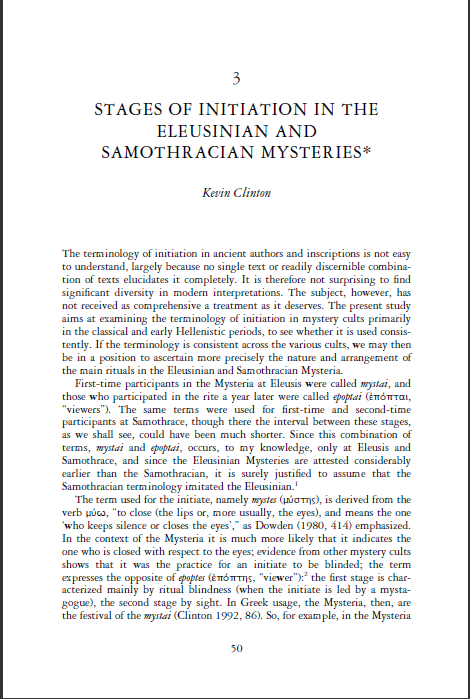
\includegraphics[width=0.6\textwidth]{./chapters/chapter38}
\end{figure}

=======


%%%%%%%%%%%%%%%%%%%%%%%%%%%%%%%%%%%%%%%%%%%
%%%%%%  STYLE 38
%%%%%%%%%%%%%%%%%%%%%%%%%%%%%%%%%%%%%%%%%%%

\cxset{style38/.style={
 name=,
 numbering=arabic,
 number font-size=\huge,
 number font-family=\rmfamily,
 number font-weight=\normalfont,
 number before={\begin{center}},
 number position=leftname,
 chapter font-family=\sffamily,
 chapter font-weight=\normalfont,
 number after={\vspace*{6.5pt}\par},
 chapter before={},
 chapter after={},
 chapter color={black!90},
 number color=\color{black!90},
 title beforeskip={},
 title afterskip={\vspace{50pt}},
 title before=,
 title after={\par\end{center}} ,
 title font-family=\rmfamily,
 title font-color=\color{black!80},
 title font-weight=\normalfont,
 title font-size=\huge,
 chapter font-size=,
}}

\cxset{style38,
       author block=true,
       author block format=\centering}
\chapter{STAGES OF INITIATION IN THE\\ ELEUSINIAN AND\\ SAMOTHRACIAN MYSTERIES\\STYLE 38}

This style uses rules to enclose both the chapter name and number as well as the title, which necessarily needs to be rather short.
\medskip

\begin{figure}[ht]
\centering
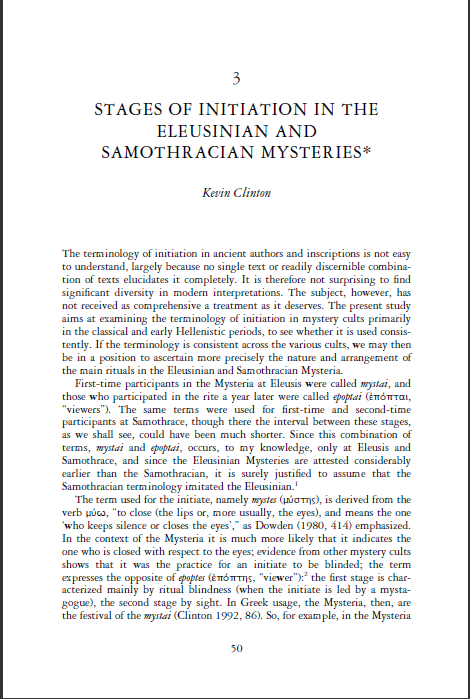
\includegraphics[width=0.6\textwidth]{./chapters/chapter38}
\end{figure}

>>>>>>> merged

\chapter{Test}
\cxset{epigraph align=center, 
       epigraph text align=center,
       epigraph source align=center}
\expandafter\epigraph{Any tikzpicture is considered like a character in LaTeX. There is no fixed relation between tikzpicture coordinates and the printed page.}{yiannis}
\lipsum
\section{Test}
\lipsum
\subsection{Test}
\lipsum
\subsubsection{Test}
\lipsum

\CMDI{\tex} can be used to set the \tex logo.
\end{document}
